\section{Proof of Concepts}

One main part of the investigation into the CERN-Solid collaboration is the development of a \gls{poc}. The \gls{poc} contains the creation of two independent software modules in an existing system from \gls{cern}. These software modules should show how it is to develop with the Solid principles in mind and to the Solid standard.

The goal of these modules is the symbiosis of decentralized stored data in a highly functional system without comprising its performance, security, or usability.

\subsection{POC 1: Commenting Module for Events in Indico}

The first \gls{poc} is supposed to enrich the Indico system with some sort of Solid-based content. With the product owner and chief developer of Indico, the CERN-Solid project manager and a Solid developer it was decided a commenting module for Indico events is an adequate solution to include data from an external storage entity namely a data pod. The ability to allow users of Indico to leave a comment on an event, which then lives in a data pod completely controlled by the author of the comment was concluded to be an attractive feature for Indico.

\begin{figure}
    \centering
    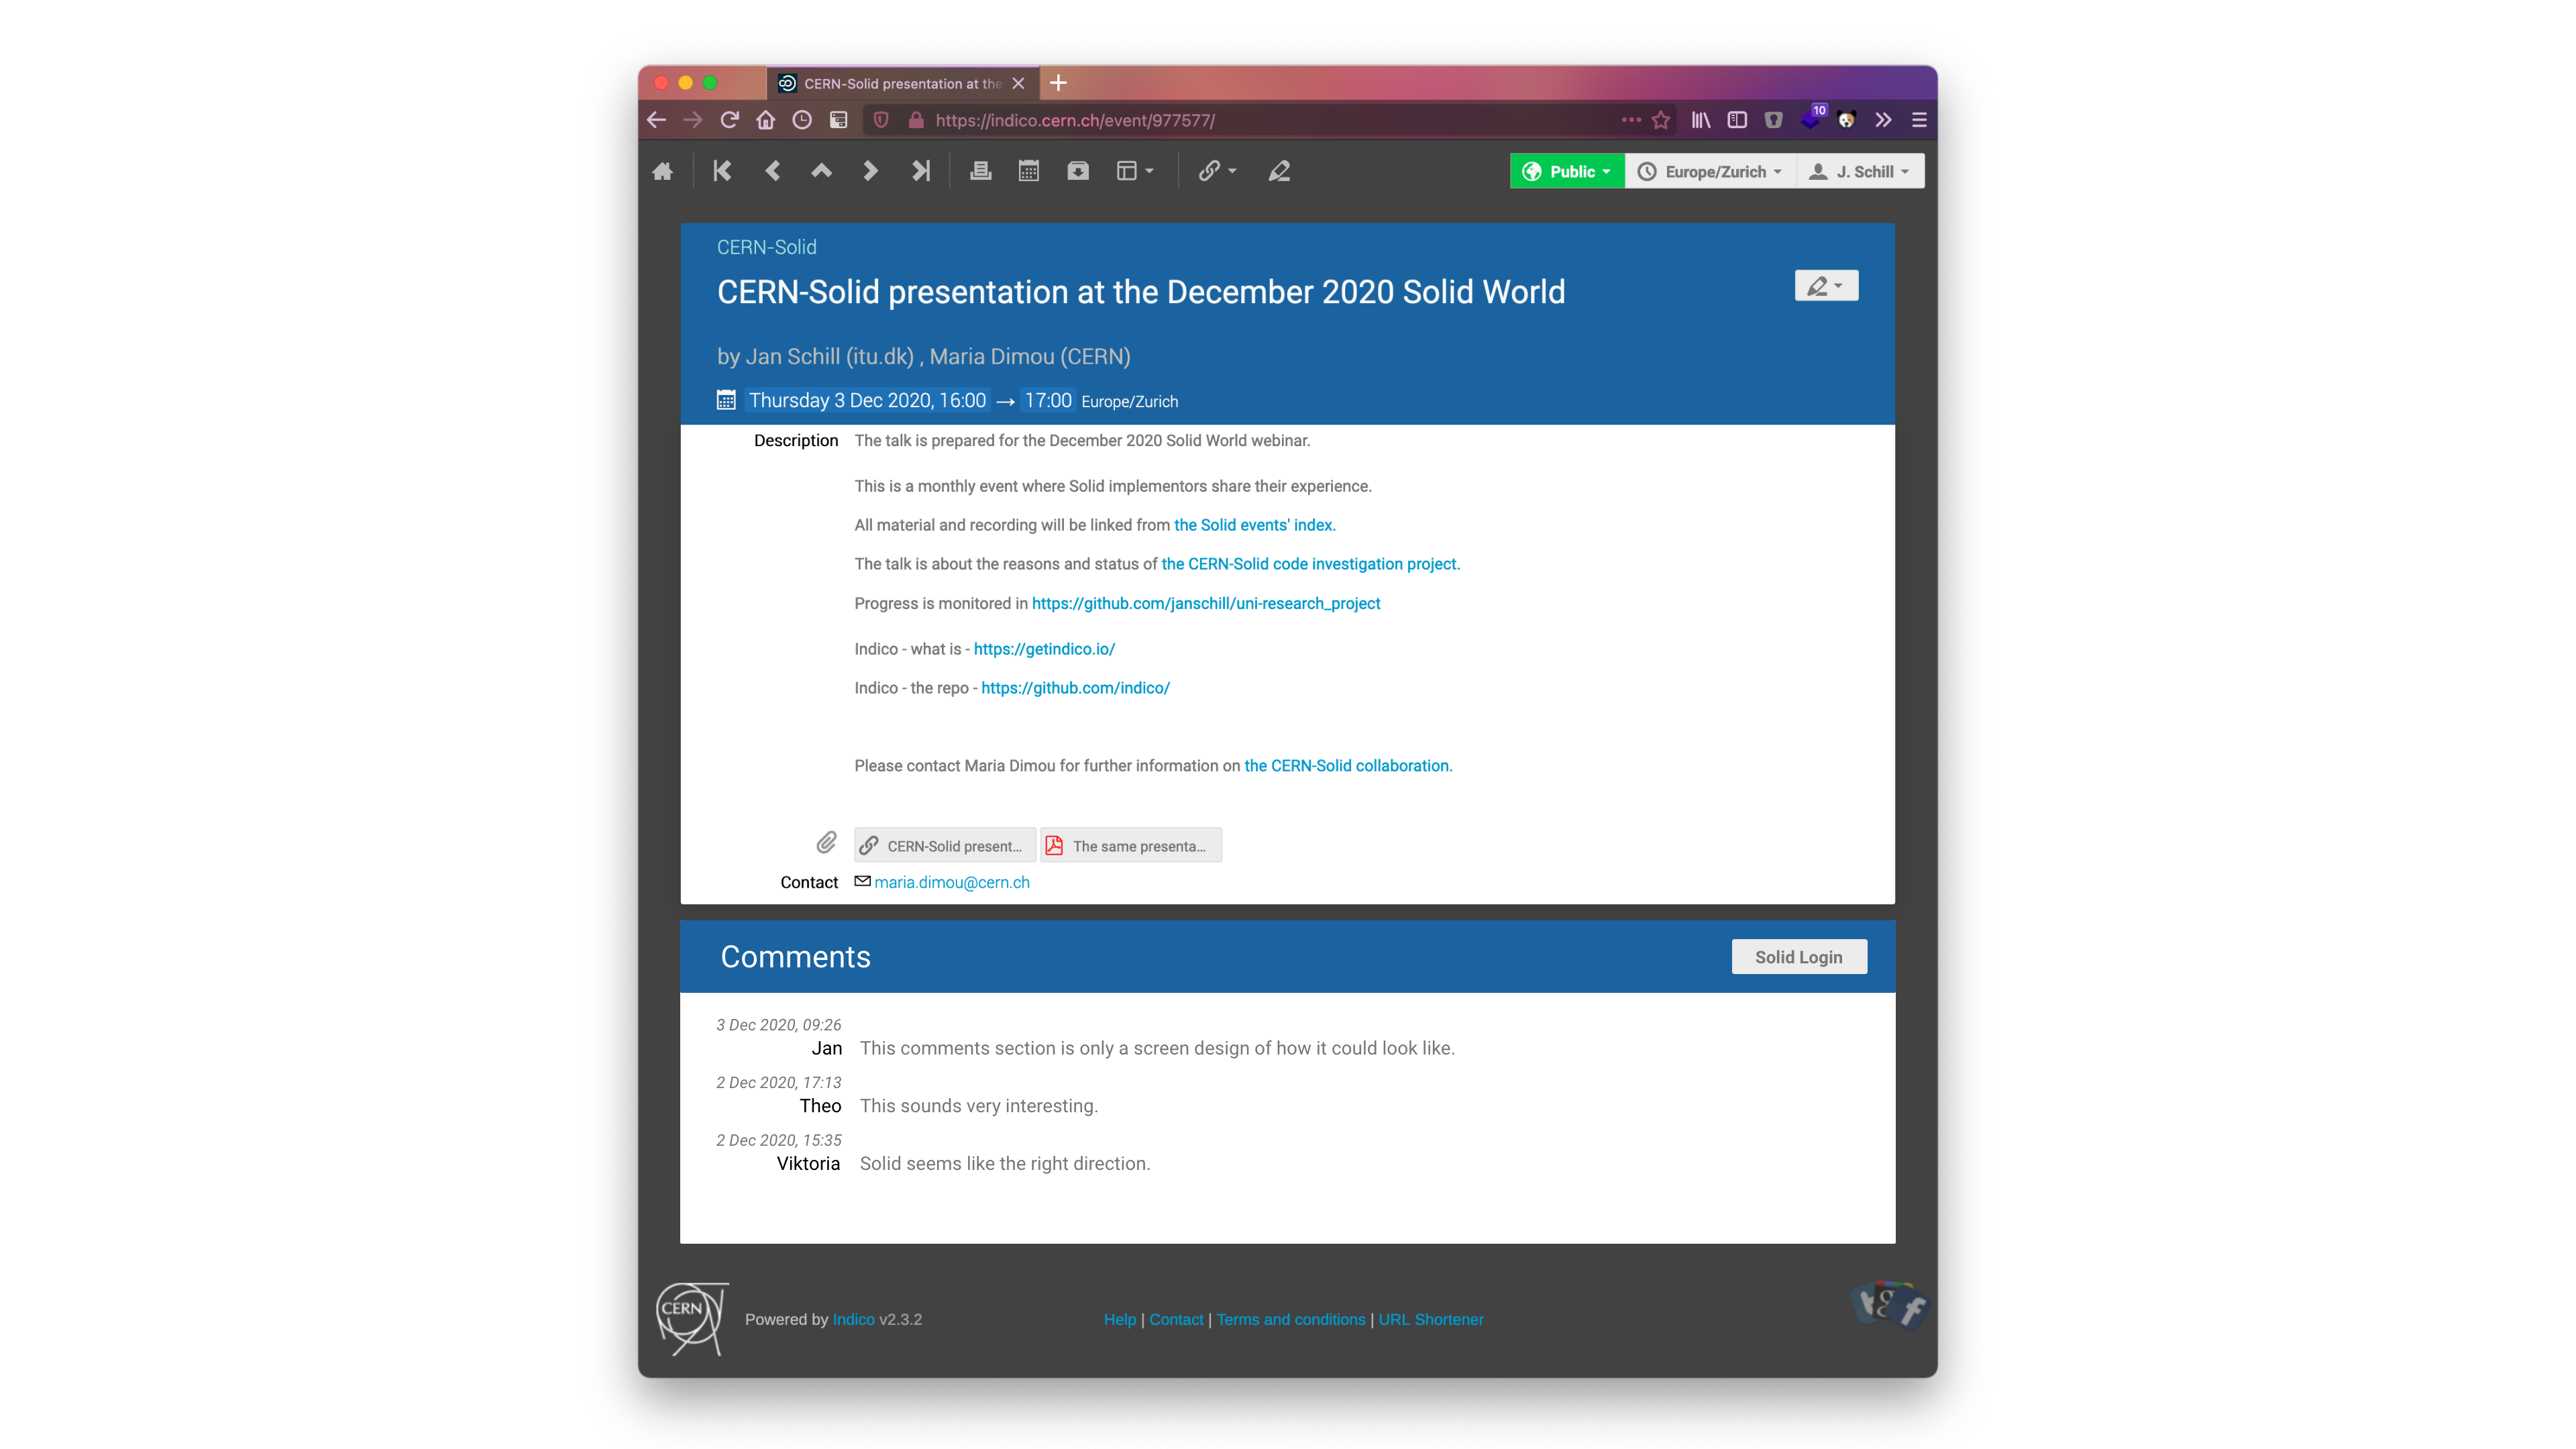
\includegraphics[width=1\textwidth]{prototype/screen_design/indico-comments-screen_design.png}
    \caption{User interface showing the comment module.}
    \label{fig:indico-comments-screen_design}
\end{figure}

\subsubsection{Design}\mbox{}\\

For the implementation of this module several design decisions had to be made. From the fundamental choice of the module running on the client device or be computed on the server and then propagated to the client afterwards or even with a microservice proxying all traffic through it to enable Solid without changing Indico.
Other design challenges were around how to protect the resources holding the comment information. These resources reside on the external data pod and need to be fetched from the application and read by other agents. Can \glspl{acl} be configured to allow the specific use-case?

\paragraph{Client- versus Server-Side versus Microservice}\mbox{}\\

When an agent browses to a running instance of Indico most of the functionality is being prepared on the server hosting Indico. It retrieves the specific request, builds the \gls{html}, and sends it to the user. For Indico most of the functionality is built with Python and the web framework Flask. Sometimes functionality needs to be closer to the user, an example is dynamic rendering of \gls{dom} elements. This is useful when new data needs to be shown right away without getting the blank white screen on a page reload.
Indico does send JavaScript, which is used for client-side features, but it focuses on keeping most its features on the server.

To make the right decision if the module should be primarily developed for the client- or server-side or even as a microservice, a list of requirements to the module had to be defined. With the defined requirements in place it had to be figured out how much functionality can be extracted from existing libraries and how much needed to be implemented with the new module. Implementing existing functionality for a new programming language would defeat the \gls{poc}’s purpose of showing how an existing software could work with the Solid principles.

The rudimentary set of features to enable commenting for users in Indico while saving the data in a data pod includes: 

\begin{enumerate}
    \item Authentication with a Solid \gls{idp}
    \item (Authenticated) Requests to a data pod
    \item Parsing of structured data (Linked Data)
\end{enumerate}

\paragraph{Client Approach}\mbox{}\\

The module runs in the browser and is therefore written in JavaScript. A programming language which compiles to JavaScript, such as TypeScript, is also possible. This means Indico remains mostly untouched, but would have to serve the needed JavaScript to the client on traffic to an event endpoint where the comment module is integrated.

\begin{table}[h!]
    \centering
    \begin{tabular}{| l | l |} 
     \hline
     Problem & Solution \\
     \hline
      Language & JavaScript or TypeScript  \\
      Framework & Native JavaScript  \\
      Client & solid-client-js \cite{solid-client-js}  \\
      Authentication & solid-client-authn-browser \cite{solid-client-authn-browser} \\
      RDF & solid-common-vocab-js \cite{solid-common-vocab-js}, rdflib.js \cite{rdflib.js}  \\
     \hline
    \end{tabular}
    \vspace{0.75cm}
    \caption{Existing solutions to problems for a client approach.}
    \label{table:1}
\end{table}

The communication flow with the data pod and the module would happen primarily from the browser.

\begin{figure}[H]
    \centering
    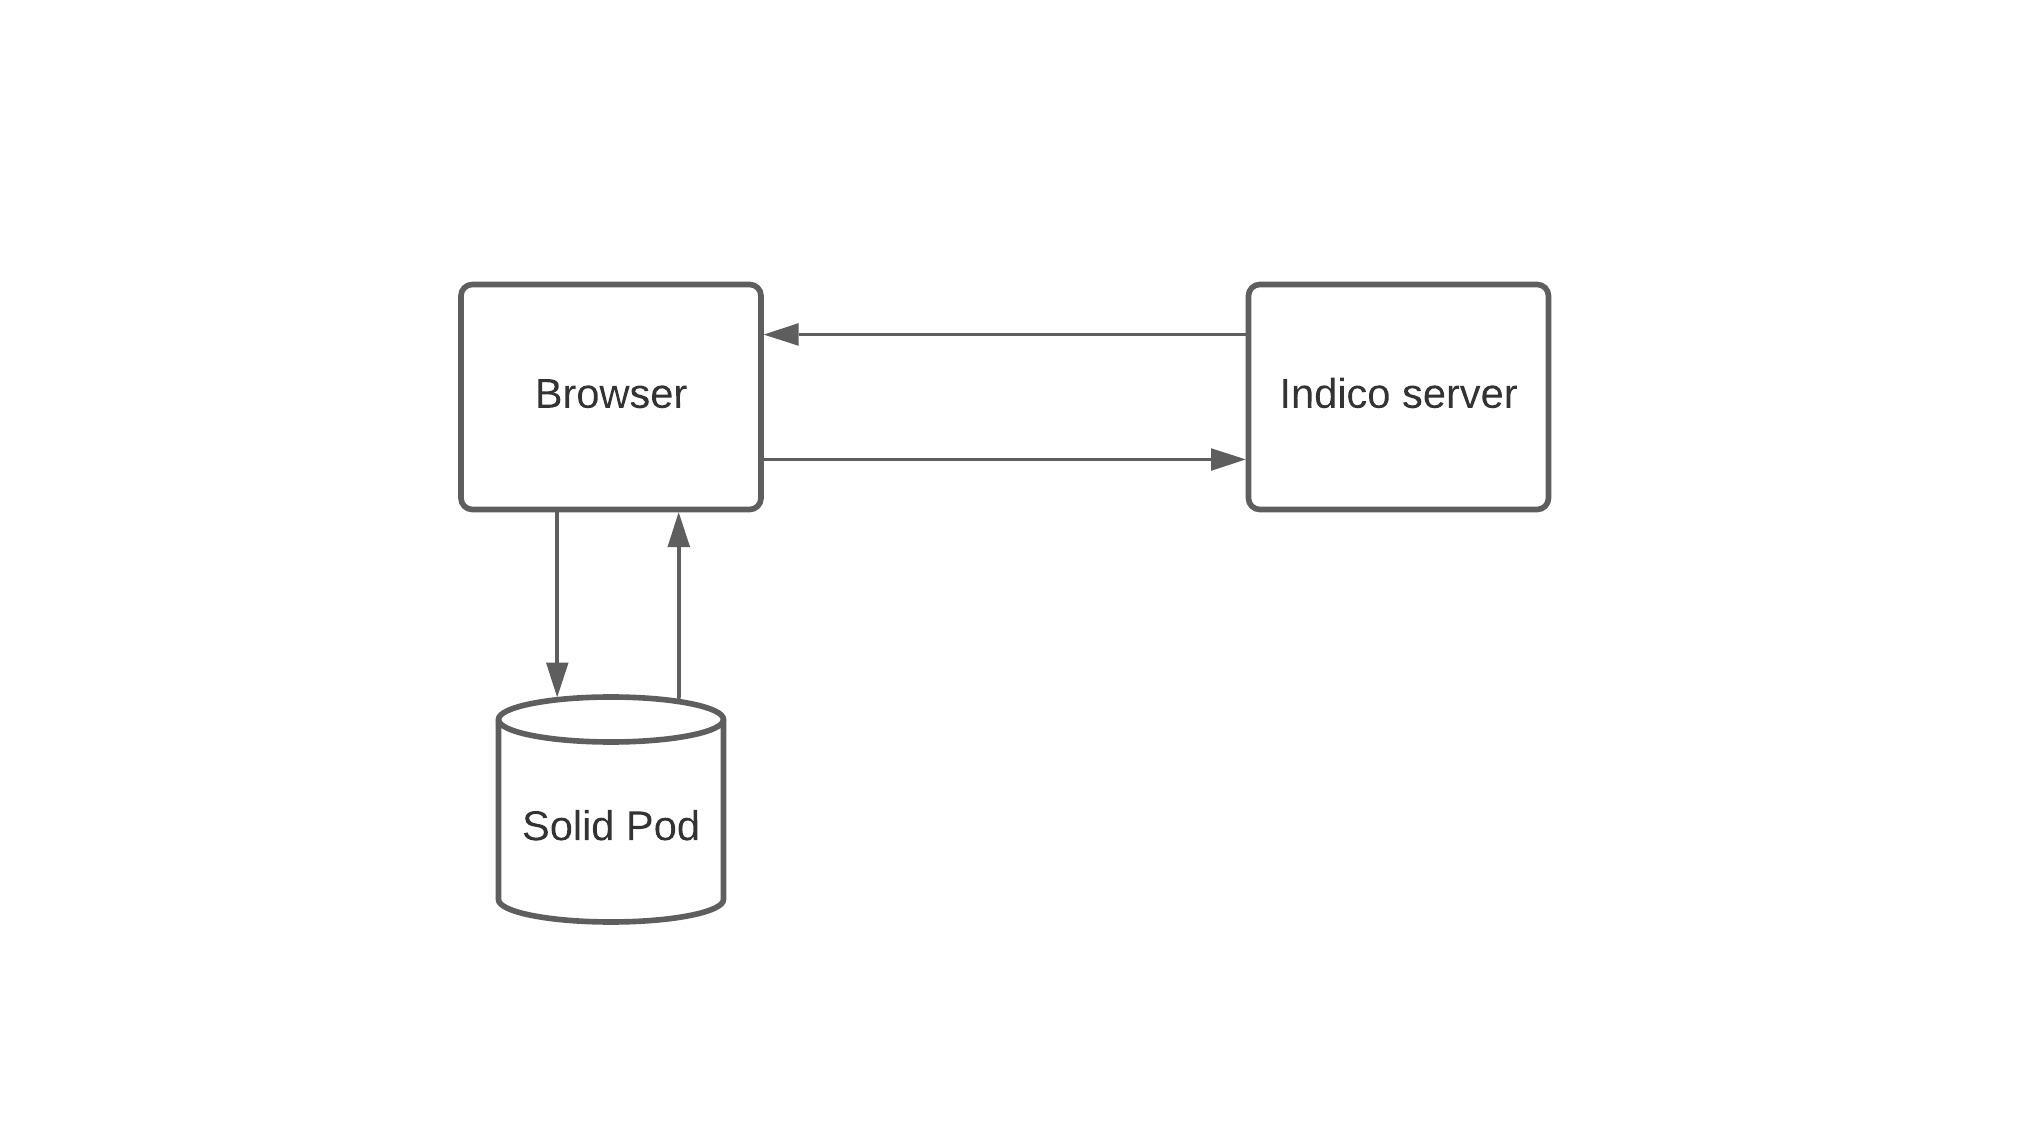
\includegraphics[width=0.8\textwidth]{prototype/graphs/poc-infrastructure-frontend.jpeg}
    \caption{Communication flow for a module developed on the client.}
    \label{fig:poc-infrastructure-frontend}
\end{figure}

\paragraph{Microservice Approach}\mbox{}\\

The microservice approach would allow developing the needed Solid logic on a separate service, which proxies all Solid related traffic through it an enable the Solid functionality. Most of the libraries from the client implementation can be used as well, as both developments would be written in JavaScript. Only the authentication flow would work a bit different.

\begin{table}[h!]
    \centering
    \begin{tabular}{| l | l |} 
    \hline
     Problem & Solution \\
     \hline
      Language & JavaScript or TypeScript  \\
      Framework & Node.js  \\
      Client & solid-client-js \cite{solid-client-js}  \\
      Authentication & solid-client-authn-node \cite{solid-client-authn-node} \\
      RDF & solid-common-vocab-js \cite{solid-common-vocab-js}, rdflib.js \cite{rdflib.js}  \\
    \hline
    \end{tabular}
    \vspace{0.75cm}
    \caption{Existing solutions to problems for a microservice approach.}
    \label{table:2}
\end{table}

The microservice module would handle take all requests aimed at the data pod and make it compliant with the Solid server. It would provide the client with the proper \gls{solidoidc} flow to attach the access token to all authenticated requests.

\begin{figure}[H]
    \centering
    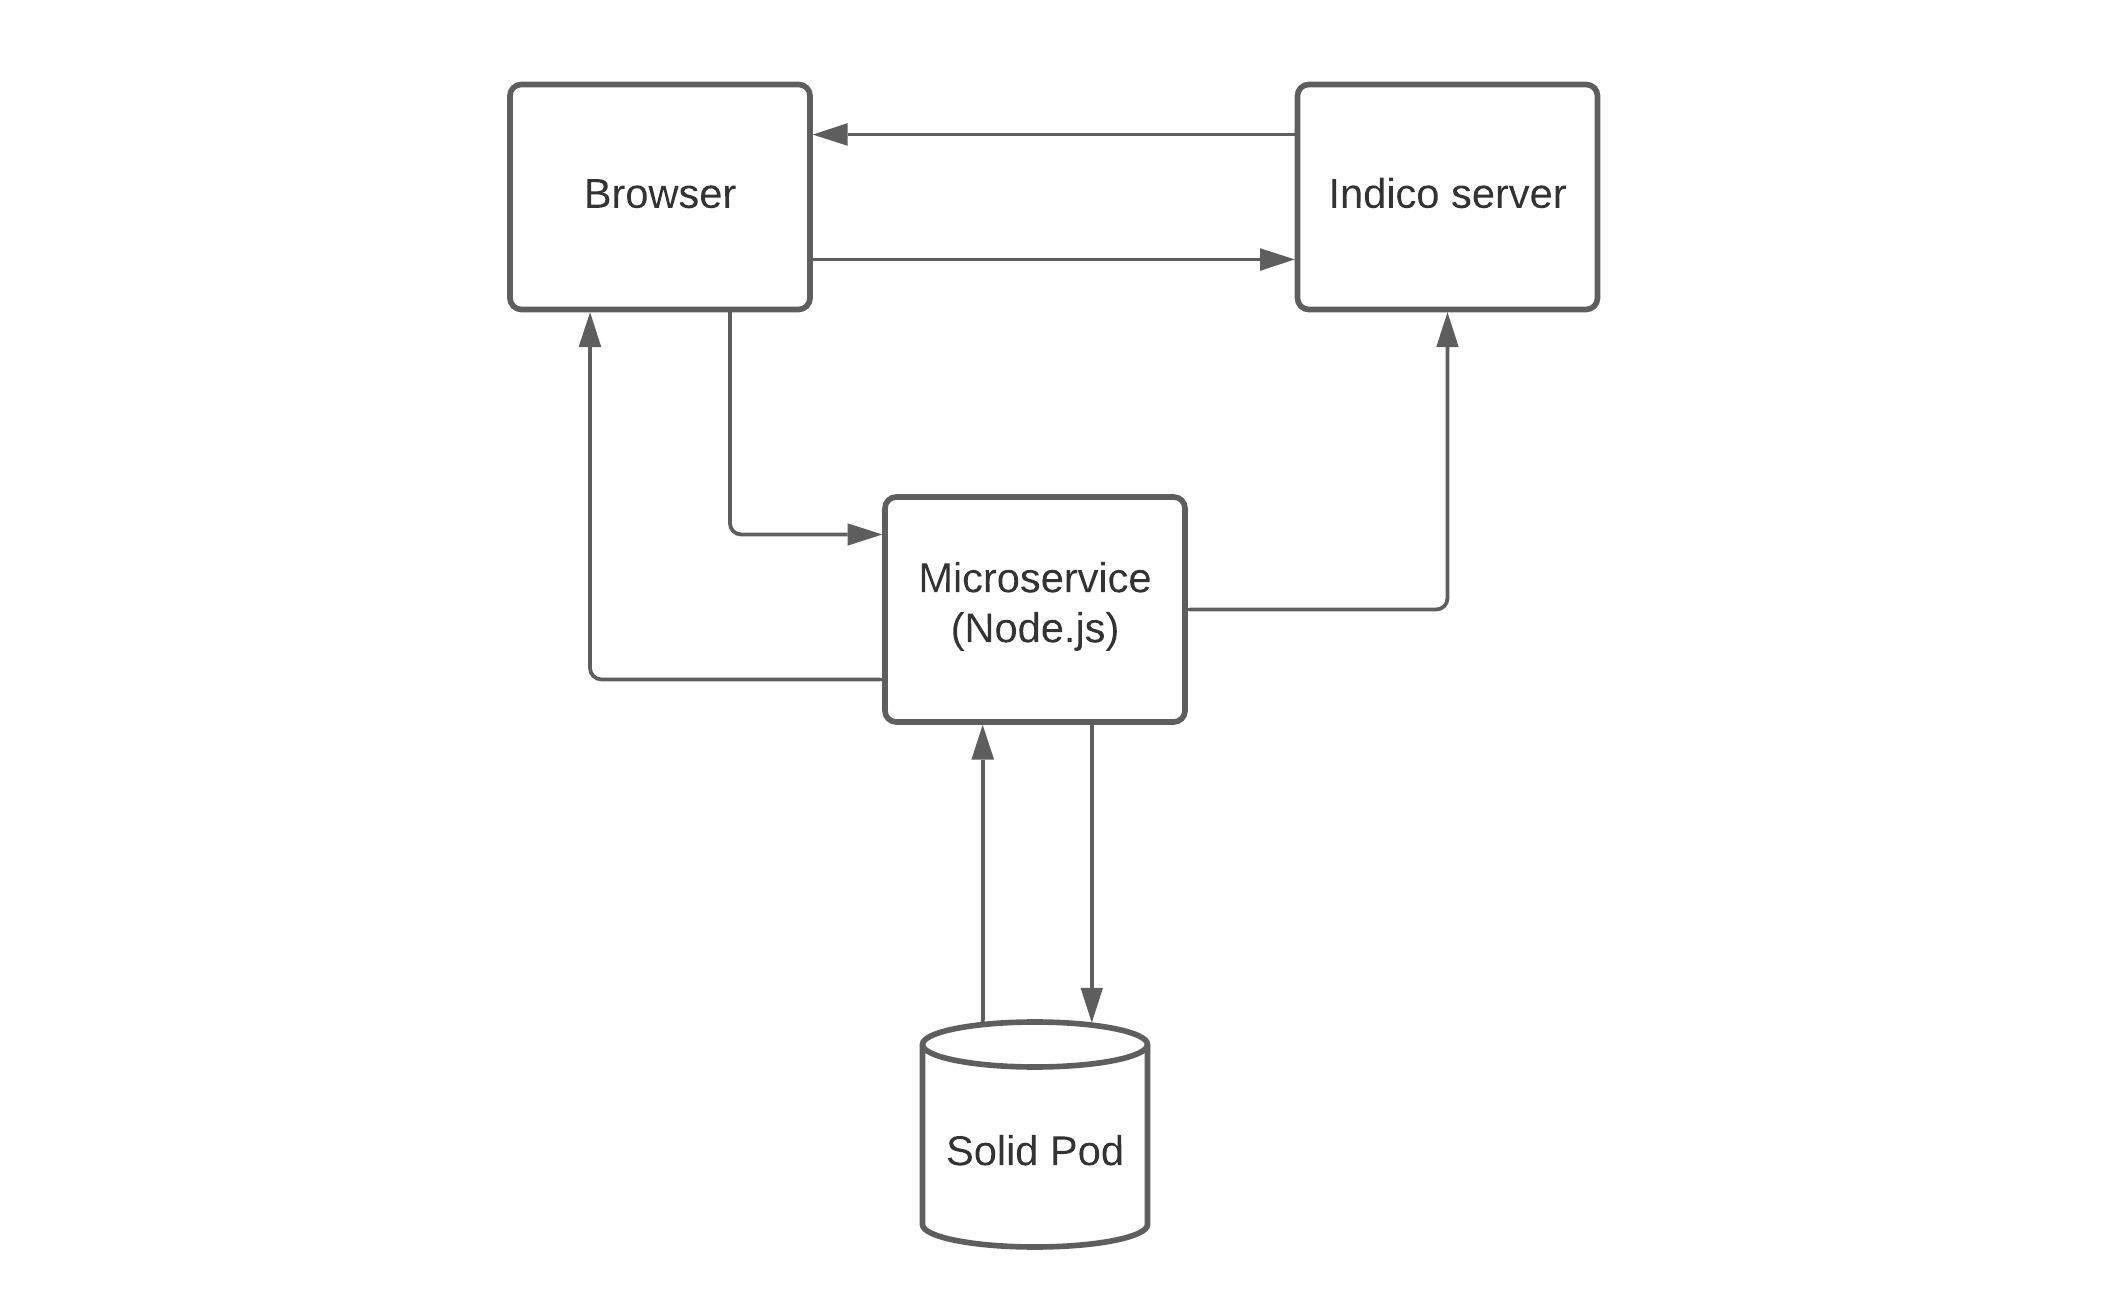
\includegraphics[width=0.8\textwidth]{prototype/graphs/poc-infrastructure-microservice.jpeg}
    \caption{Communication flow for a module developed as a microservice.}
    \label{fig:poc-infrastructure-microservice}
\end{figure}

\paragraph{Server Approach}\mbox{}\\

Goal of the server approach would be just like with the microservice approach to decouple the logic needed to work with Solid from the client and have it run on a server instance. The attractiveness for the server approach would be it could be fully integrated within Indico and be part of its Python code base. The major drawbacks are no direct Solid libraries written in Python exist to allow a seamless integration into the ecosystem.

\begin{table}[!ht]
    \centering
    \begin{tabular}{| l | l |} 
    \hline
     Problem & Solution \\
     \hline
      Language & Python  \\
      Framework & Flask  \\
      Client & -  \\
      Authentication & pyoidc \cite{pyoidc} missing DPoP\\
      RDF & solid-common-vocab-js \cite{solid-common-vocab-js}, rdflib.js \cite{rdflib.js}  \\
    \hline
    \end{tabular}
    \vspace{0.75cm}
    \caption{Existing solutions to problems for a server approach.}
    \label{table:3}
\end{table}

The authentication library pyoidc allows authenticating with \gls{oidc} systems, but is missing a mandatory feature called \gls{dpop}, which is needed to make requests to protected resources on a data pod.

\begin{figure}
    \centering
    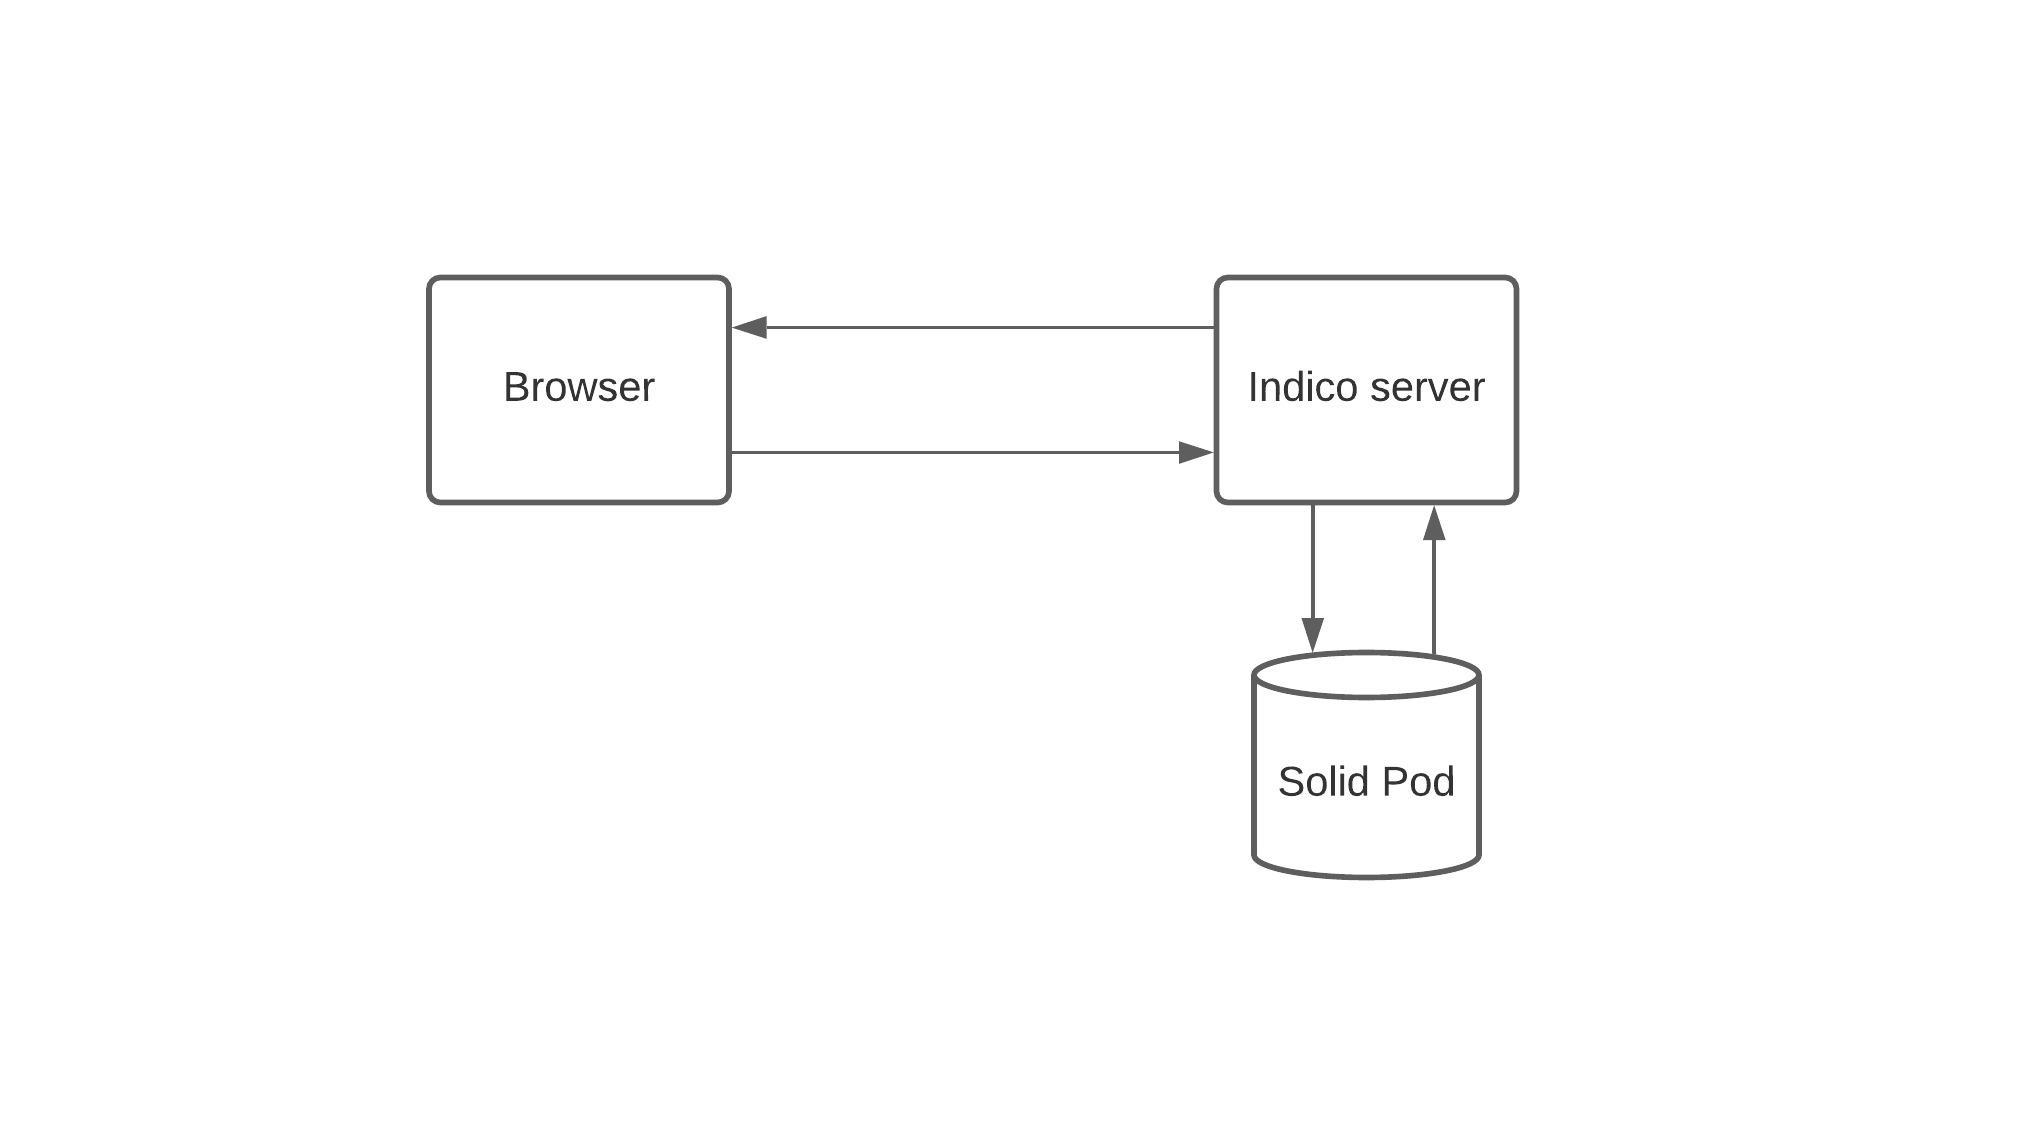
\includegraphics[width=0.8\textwidth]{prototype/graphs/poc-infrastructure-backend.jpeg}
    \caption{Communication flow for a module developed on the server.}
    \label{fig:poc-infrastructure-backend}
\end{figure}

\paragraph{Comparison of the Different Approaches}\mbox{}\\

Benefits from developing the module for the client:

\begin{itemize}
    \item Necessary libraries exist (Major release for all basic Solid flows exist)
    \item Community support
    \item Programming effort for an \gls{mvp} lowest
    \item Documentation on developing Solid apps in JavaScript exist
\end{itemize}


\begin{table}[h!]
    \centering
    \begin{tabular}{| l | p{11cm} |} 
    \hline
     Library & Description \\
     \hline
      solid-client & A client library for accessing data stored in Solid Pods.  \\
      \hline
      solid-client-authn & A set of libraries for authenticating to Solid identity servers:solid-client-authn-browser for use in a browser.solid-client-authn-node for use in Node.js.  \\
      \hline
      vocab-common-rdf & A library providing convenience objects for many RDF-related identifiers, such as the Person and familyName identifiers from the Schema.org vocabulary from Google, Microsoft and Yahoo!  \\
      \hline
      vocab-solid-common & A library providing convenience objects for many Solid-related identifiers.  \\
      \hline
      vocab-inrupt-common & A library providing convenience objects for Inrupt-related identifiers.  \\
      \hline
    \end{tabular}
    \vspace{0.75cm}
    \caption{Existing solutions to problems for a server approach.}
    \label{table:2}
\end{table}

\paragraph{Single versus Multiple Resource(s) for Comments}\mbox{}\\

Storing the comments in \gls{rdf} can be done in two ways: storing it in one file as a graph with a list of comments, or creating a file for every comment.

\begin{figure}
    \centering
    \begin{subfigure}{.5\textwidth}
      \centering
      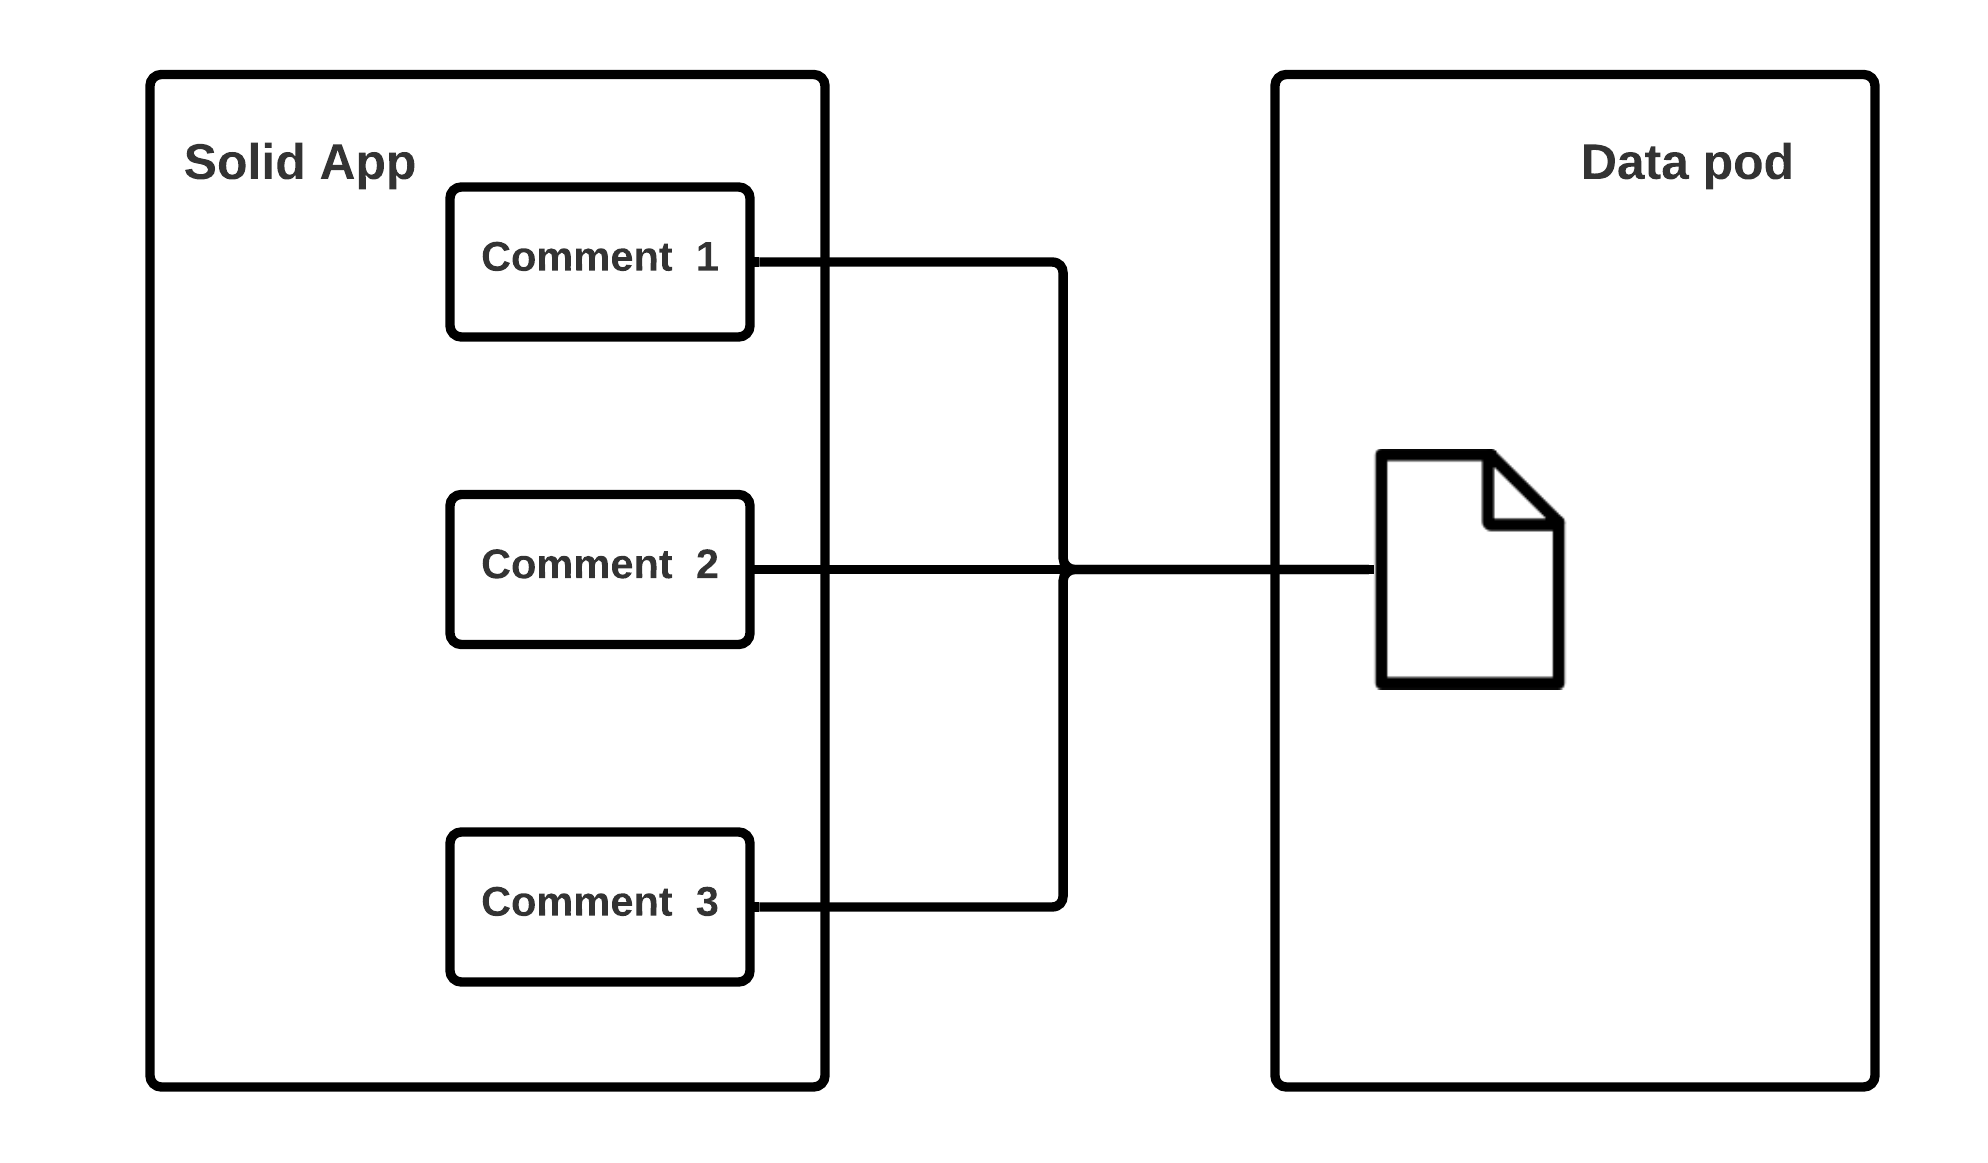
\includegraphics[width=0.7\textwidth]{prototype/graphs/poc-comment-single-resource-comments.png}
      \caption{TODO: caption}
      \label{fig:ppc-comment-single-resource-comments}
    \end{subfigure}%
    \begin{subfigure}{.5\textwidth}
      \centering
      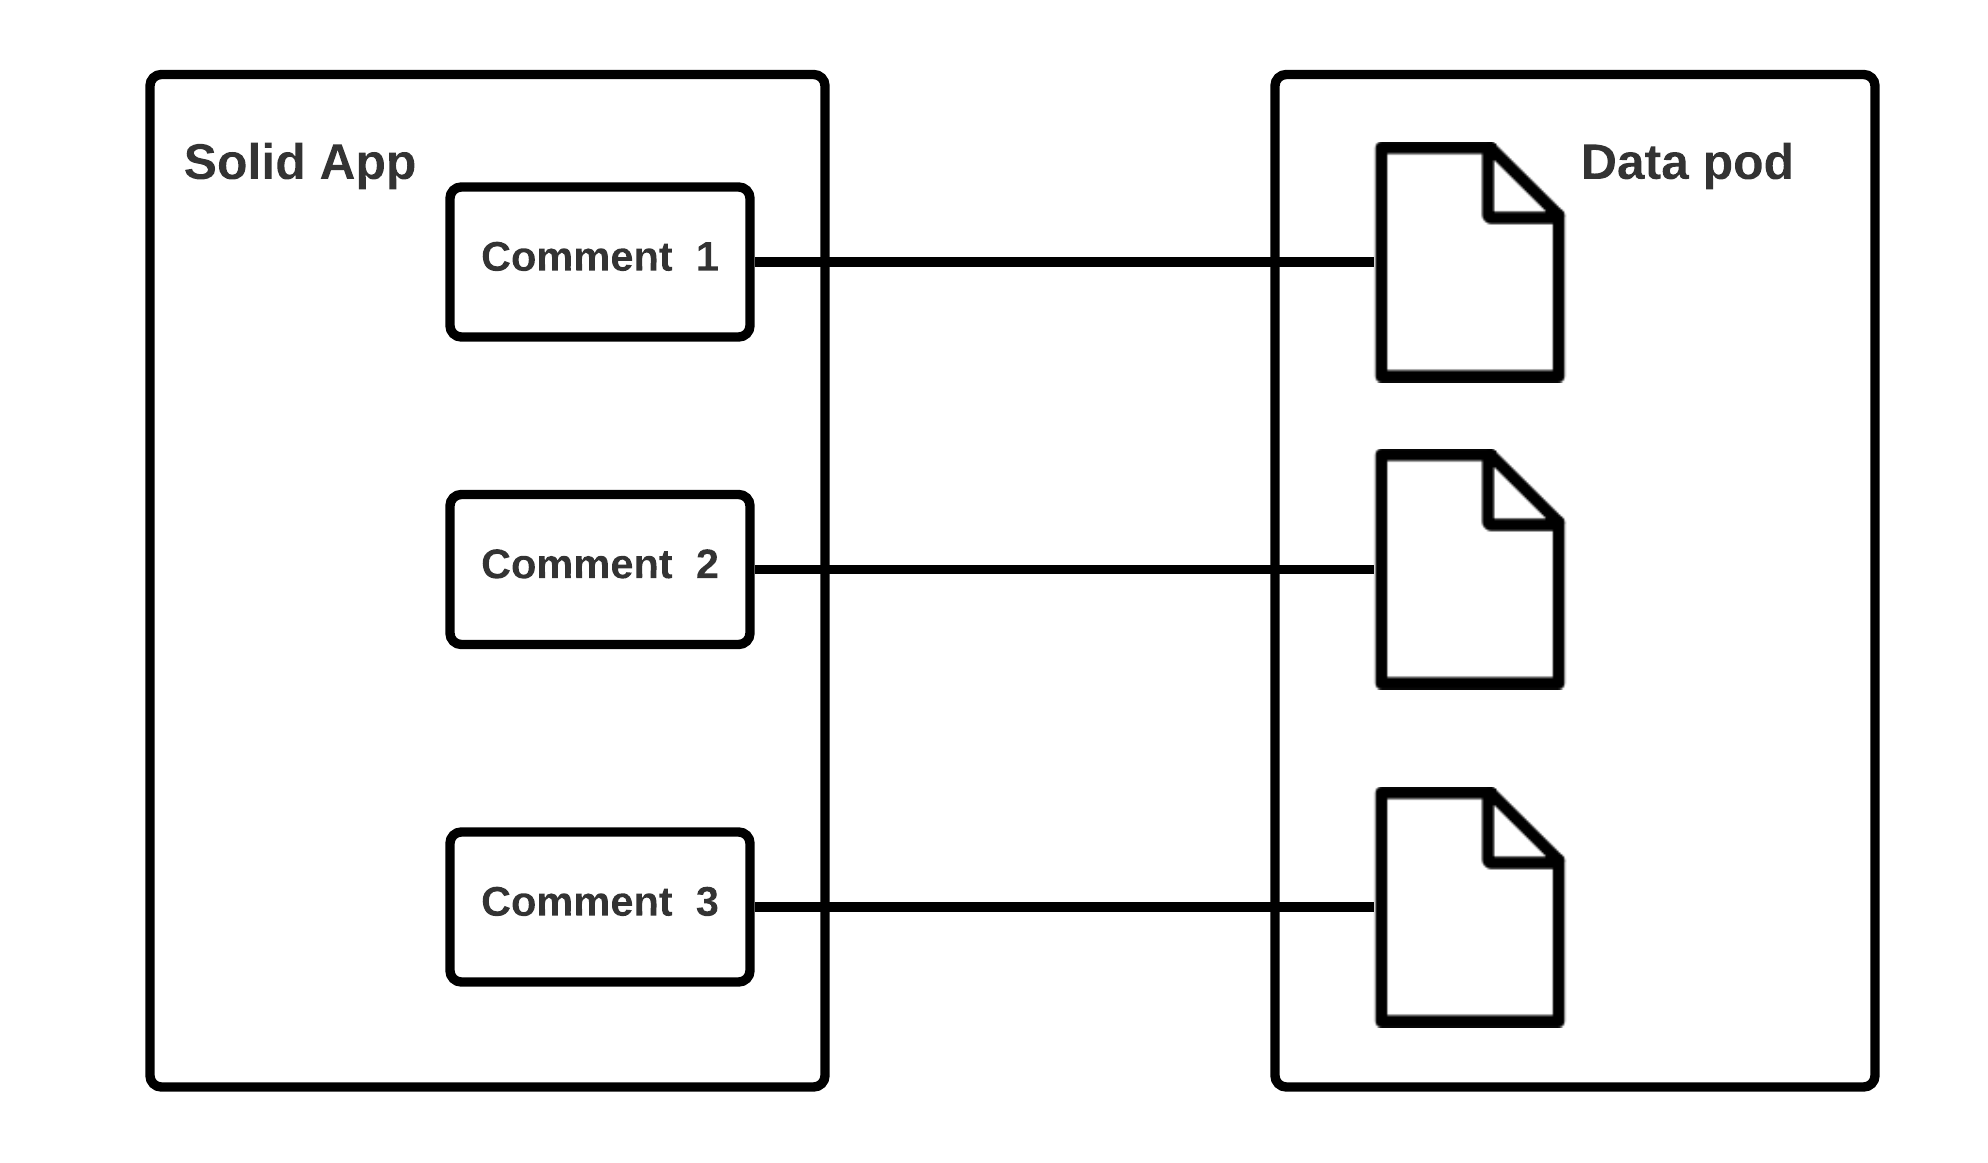
\includegraphics[width=0.7\textwidth]{prototype/graphs/poc-comment-multiple-resources-comments.png}
      \caption{TODO: caption}
      \label{fig:poc-comment-multiple-resources-comments}
    \end{subfigure}
    \caption{TODO: two approaches}
    \label{fig:test}
\end{figure}

When fetching the container with all the comment resources the request returns a Turtle file describing the container, but not the actual content of the contained resources. The misconception of receiving the content as well, was thought to be a problem, as it was assumed an initial request to the container reading its child resources had to be made and then for each resource a request needed to be built to retrieve the resource. This overhead was later disproved as the application where this module is embedded maintains the list of resources to be fetched. Therefore, no manual building of requests to those resources had to be done. The next paragraph also lays out how this design would not work with the protection of the resources.

\paragraph{Protection on Resource}\label{protection-on-resource}\mbox{}\\

Every container and resource in Solid is protected with \gls{wac}, which determines if specific agents, groups, or the world can have read, write, append, or control access. These control access modes are defined in \gls{acl} files. The Solid \gls{acl} inheritance algorithm looks for an \gls{acl} file attached to a specific resource, if it cannot find one it goes recursively up the file hierarchy and looks for \glspl{acl} on the containers.
Indico allows two general types of protection \textit{private} and \textit{public} on its events. Public means open to everyone, no Indico account or any type of authorization is needed to see the event. Whereas private can be as fine-grained as only to specific agents or groups. A comment module is only valuable if the comments can be read by anyone and be written by authorized users.

In order for visitors of a private or public event in Indico to be able to see the comment, the comment’s \gls{acl} needs to allow the public to read the resource. This can be achieved by using the \textit{public} container, which comes with public-read by default on the \gls{nss} or by creating a new container and setting the \gls{acl} with:

\begin{lstlisting}[language=Other,columns=fullflexible, caption={TODO: Label caption}, label={lst:1}]
@prefix acl: <http://www.w3.org/ns/auth/acl#>.
@prefix foaf: <http://xmlns.com/foaf/0.1/>.

# ... Definition for owner

<#example-container-name>
    a acl:Authorization;
    acl:agentClass foaf:Agent;
    acl:accessTo <./>;
    acl:mode acl:Read.
\end{lstlisting}

Every resource in this container is by definition readable by the public -- if not otherwise stated in a more detailed resource \gls{acl}. The above definition even allows the reading of the container’s content, meaning a request to the container would yield a list of resources in the container. This becomes unpleasant if the Indico event is private and the comments for this Indico event should not be read by the world, which is entirely possible, when browsing to the location of a specific data pod and then looking into the public container.

To prevent a random agent to see the contents of a container, the container can be set to private, with the container’s resources to still be public. This would allow everyone provided they have the \gls{url} to browse to the public resource and read it, but not look into the resource’s parent container. To achieve this behavior with \gls{acl}, the container needs to just define its owner and no specific rules for the public, as \gls{wac} comes with a default private access control. Each child resource needs to define an \gls{acl} now, allowing public read.
The container’s \gls{acl} would look like the following with just a owner defined:

\begin{lstlisting}[language=Other,columns=fullflexible, caption={TODO: Label caption}, label={lst:2}]
@prefix acl: <http://www.w3.org/ns/auth/acl#>.

<#owner>
    a acl:Authorization;
    acl:agent <https://janschill.net/profile/card#me>;
    acl:accessTo <./>;
    acl:default <./>;
    acl:mode acl:Read, acl:Write, acl:Control.
\end{lstlisting}

A child resource would allow public read with:

\begin{lstlisting}[language=Other,columns=fullflexible, caption={TODO: Label caption}, label={lst:3}]
@prefix : <#>.
@prefix acl: <http://www.w3.org/ns/auth/acl#>.
@prefix foaf: <http://xmlns.com/foaf/0.1/>.

# ... Definition for owner

:Read
    a acl:Authorization;
    acl:accessTo <test.txt>;
    acl:agentClass foaf:Agent;
    acl:mode n0:Read.
\end{lstlisting}

Another approach and the one implemented after iterating through the previous ones is to have the container’s \gls{acl} resource define a default access mode for its child resources. This way one \gls{acl} only needs to be created on the container and all resources have proper access modes for public read and are not listed publicly in the container’s description.

\begin{lstlisting}[language=Other,columns=fullflexible, caption={TODO: Label caption}, label={lst:4}]
@prefix acl: <http://www.w3.org/ns/auth/acl#>.
@prefix foaf: <http://xmlns.com/foaf/0.1/>.
@prefix target: <./>.

:ReadDefault
    a acl:Authorization;
    acl:default target:;
    acl:agentClass foaf:Agent;
    acl:mode acl:Read.
\end{lstlisting}

\paragraph{Preventing Resources From Unwanted Discovery}\mbox{}\\

With the resources having proper access modes but being publicly readable a simple naming convention of taking the \gls{iso} 8601 string and using it as a filename for the resources created on the data pod does not suffice -- even though it is a good strategy when looking for a reliable naming convention to prevent duplication. Considering performance improvements such as pagination for future iterations of the module, which would require some sort of iterative indication, a combination of randomness, but also a order indicator it was settled for using \gls{uuid} plus the \gls{iso} 8601 string to form a filename.

Other ideas included hashing a random string with the timestamp to generate non-guessable filenames. The filename would need to use the same hash function to decipher the filename to figure out when the comment was generated. \gls{uuid} is a reliable and easy to use system to generate \textit{truly} globally unique strings. 

\paragraph{Modification of Resource from Data Pod}\mbox{}\\

\paragraph{Mitigation of Spam}\mbox{}\\

Enabling user input in form of comment module without application authentication is a gateway to spam. Even though authentication with a Solid \gls{idp} is necessary, it does not hinder a malicious actor to create a multitude of Solid accounts and spam into the application. In the first iteration of the module only Solid authentication was integrated into the module and would therefore allow anyone with a Solid account to post comments and thus also spam the Indico event theoretically. In a second iteration of the module another authentication layer was added to mitigate spam from outside of Indico. For \gls{cern}’s use-case an authenticated Indico session was enough. This adds an extra step to the comment process and it is ensured only registered Indico users can comment.

\paragraph{Giving Application Full Control of Data Pod}\mbox{}\\

To create or change programmatically \glspl{acl} requires \textit{control} access to the container. By default \gls{nss} asks for the permissions when authenticating for the first time in the \gls{solidoidc} flow between the \textit{solid-comment} module and Solid \gls{idp}. The permissions granted to the application are on the root container of the data pod. Meaning, giving an application control access allows the application to read, write, change \glspl{acl} on the entire data pod. This is obviously troubling, as a simple application as a commenting module need to have control access to set the needed \glspl{acl} for the containers and resources it creates.

The current implementation has not a built-in solution, but one way of solving it, is the use of an application launcher, which is an application itself with full control access and then limits the access controls of the \textit{solid-comment} module by creating a dedicated container for it and setting the needed \gls{acl} for this specific container only.

\subsubsection{Integration with Indico}



\paragraph{Storing Reference to Comments in Indico}

\paragraph{Enforce Authenticated Session for Posting Comments}

\subsubsection{Evaluation}



\paragraph{System Description}
\paragraph{Context Diagram}
\paragraph{Stakeholders}
\paragraph{Drivers}
\paragraph{Metrics}
\paragraph{Levels}
\paragraph{Components}

\subsubsection{Analysis}

\subsection{POC 2: Auto-Complete for Conference Registration in Indico}

\subsubsection{Design}

TODO:
1st iteration, save data in pod
2nd iteration, only pull data from pod

\paragraph{Modification of Resource from Data Pod}

\paragraph{Payment on Input Fields}

\paragraph{Performance of Large Conference}

\paragraph{Availability of Crucial User Data}

\subsubsection{Integration with Indico}

\paragraph{Bind to Dynamically Created Form}

\subsubsection{Evaluation}

\paragraph{System Description}
\paragraph{Context Diagram}
\paragraph{Stakeholders}
\paragraph{Drivers}
\paragraph{Metrics}
\paragraph{Levels}
\paragraph{Components}

\subsubsection{Analysis}

\subsection{Deployment of Indico Instance}
